% !TEX program = xelatex

\documentclass[aspectratio=169]{beamer}

\usepackage{xltxtra} 
\usetheme{focus}
\XeTeXlinebreaklocale "th_TH"
\usepackage{fontspec}
\defaultfontfeatures{Mapping=tex-text,Scale=MatchLowercase}
% \setsansfont{Gillius ADF No2}
% \setmonofont{Tlwg Typist}
\usepackage{listings}
\usepackage{color}

\definecolor{codegreen}{rgb}{0,0.6,0}
\definecolor{codegray}{rgb}{0.5,0.5,0.5}
\definecolor{codepurple}{rgb}{0.58,0,0.82}
\definecolor{backcolour}{rgb}{0.95,0.95,0.92}

\lstdefinestyle{codeblock}{
    backgroundcolor=\color{backcolour},   
    commentstyle=\color{codegreen},
    keywordstyle=\color{magenta},
    numberstyle=\tiny\color{codegray},
    stringstyle=\color{codepurple},
    basicstyle=\footnotesize,
    breakatwhitespace=false,         
    breaklines=true,                 
    captionpos=b,                    
    keepspaces=true,                 
    numbers=left,                    
    numbersep=5pt,                  
    showspaces=false,                
    showstringspaces=false,
    showtabs=false,                  
    tabsize=4
}
\lstset{style=codeblock}

\usepackage{smartdiagram}

\title{First Step to Practical Machine Learning}
\subtitle{Knowledge Sharing for CPE/SKE students}
\author{Sirakorn Lamyai}
\institute{Student, Kasetsart U.}
\date{October 30, 2018}
\begin{document}

\begin{frame}
	\titlepage
\end{frame}

\begin{frame}
	\frametitle{Before we start...}
	Make sure these are installed on your computer.\\
	{\tiny This page is a guide for installing on Windows}
	
	\begin{itemize}
		\item Python 3.6: Download and install at \url{https://www.python.org}
		\item NumPy, Scipy, Matplotlib, Scikit-learn, MLxtend:\\
		Run \texttt{pip install numpy scipy matplotlib sklearn mlxtend}
	\end{itemize}
\end{frame}

\begin{frame}
	\frametitle{Outline}
	\tableofcontents
\end{frame}

\section{Introduction to Machine Learning}

\subsection{What is Machine Learning?}

\begin{frame}
	\frametitle{What is Machine Learning?}
	\pause
	\begin{figure}
		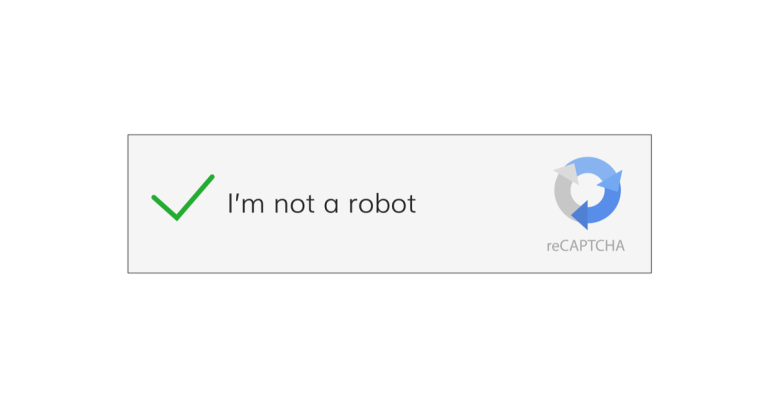
\includegraphics[scale=0.4]{imgs/recaptcha.png}
	\end{figure}
	\begin{itemize}
		\pause
		\item This is Recaptcha.
		      \begin{itemize}
			      \pause
			      \item Recaptcha helps stop millions of spam a day.
			            \pause
			      \item In some old days, we have to type Captcha texts to distinguish ourself from bots.
			            \pause
			      \item How is it possible that with a single click, an automated system can distinguish bots from humans?
		      \end{itemize}
	\end{itemize}
\end{frame}

\subsubsection{Traditional programming approach}

\begin{frame}
	\frametitle{Traditional programming approach}
	\begin{center}
		\smartdiagram[circular diagram]{Analyse, Algorithm, Test, Improve, Repeat}
	\end{center}
\end{frame}


\subsubsection{Machine learning approach}

\begin{frame}
	\frametitle{Machine learning approach}
	\begin{center}
		\smartdiagram[circular diagram]{Analyse, Machine Learning, Validation, Improve, Repeat}
	\end{center}
\end{frame}

\begin{frame}
	\frametitle{In other words...}
	\begin{center}
		Machine Learning \\
		\onslide<2-> \huge = Data + Data analysis algorithm \\
		\onslide<3-> \Huge = Adapt to change
	\end{center}
\end{frame}

\section{Machine Learning Problems}

\begin{frame}
	\frametitle{Types of Machine Learning problems}
	\begin{enumerate}
		\item<2-> Supervised learning
		\item<3-> Unsupervised learning
		\item<4-> Reinforcement learning
	\end{enumerate}
\end{frame}

\subsection{Supervised learning}

\begin{frame}
	\frametitle{Supervised learning}
	\begin{columns}
		\column{0.5\textwidth}
			\begin{figure}
				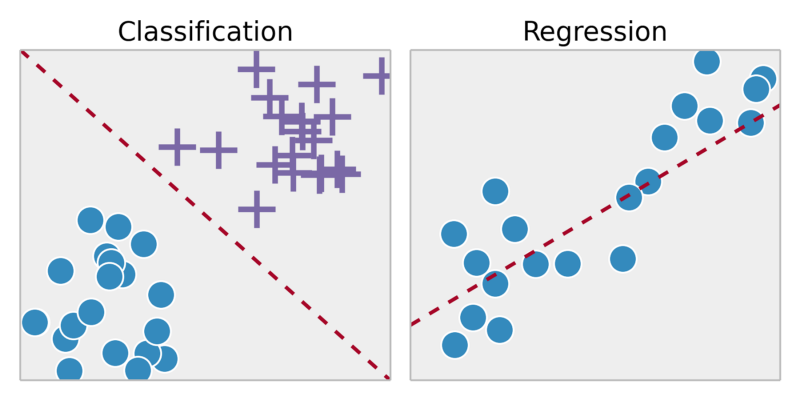
\includegraphics[width=1.0\textwidth]{imgs/supervised_learning.png}
			\end{figure}
		\column{0.5\textwidth}
			\begin{itemize}
				\item<2-> Given a \textbf{training set} for the data, find a \textbf{model} to \textbf{generalise} well to \textbf{unseen} data.
				\item<3-> Two main supervised learning problems
				\begin{itemize}
					\item<4-> Classification: On the discrete data
					\item<5-> Regression: On the continuous data
				\end{itemize}
				\item<6-> Example problems: Spam E-mail detection, Facial recognition
			\end{itemize}
	\end{columns}
\end{frame}

\subsection{Unsupervised learning}

\begin{frame}
	\frametitle{Unsupervised learning}
	\begin{columns}
		\column{0.5\textwidth}
			\begin{figure}
				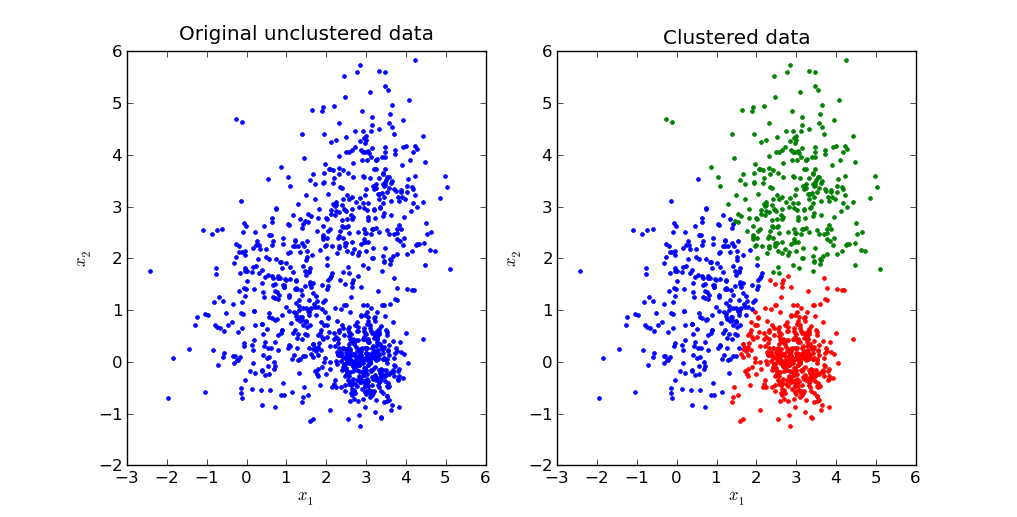
\includegraphics[width=1.0\textwidth]{imgs/kmeans.png}
			\end{figure}
		\column{0.5\textwidth}
			\begin{itemize}
				\item<2-> Discover \textbf{hidden} structure in \textbf{non-labelled} data.
				\item<3-> Example: Clustering, Generative models
			\end{itemize}
	\end{columns}
\end{frame}

\subsection{Reinforcement learning}

\begin{frame}
	\frametitle{Reinforcement learning}
	\begin{figure}
		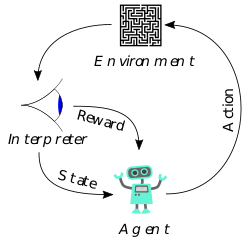
\includegraphics[scale=.7]{imgs/reinforcement_learning.png}
	\end{figure}
\end{frame}

\section{Model}

\begin{frame}
	\frametitle{Model}
	\begin{itemize}
		\item<2-> A result of the combination between...
		      \begin{itemize}
			      \item<3-> a \textbf{method} to recognise the data, and
			      \item<4-> \textbf{sample datas} for such the method
		      \end{itemize}
	\end{itemize}
	\begin{columns}
		\column<5->{0.5\textwidth}
		\begin{figure}
			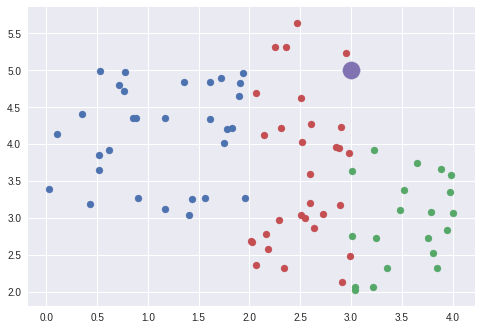
\includegraphics[scale=.3]{imgs/simple_knn.png}
		\end{figure}
		\column<6->{0.5\textwidth}
		Determine which group should the purple dot be in (red/green/blue) by \textbf{checking the colour of its nearest dot.}
	\end{columns}
	\begin{columns}
		\column{0.5\textwidth}
		\begin{center}
			\onslide<5-> \Large Data
		\end{center}
		\column{0.5\textwidth}
		\begin{center}
			\onslide<6-> \Large Method
		\end{center}
	\end{columns}
\end{frame}

\begin{frame}
    \frametitle{Beginning with our first model}
    \begin{itemize}
        \item<2-> We're going to write our \textbf{first own} machine learning algorithm called \textbf{$k$-Nearest Neighbour} ($k$-NN)
        \begin{itemize}
            \item<3-> $k$-NN is known to be very simple, with its concept as
        \end{itemize}
    \end{itemize}
    \onslide<4->
    \begin{block}{$k$-NN algorithm}
        To classify label of a data point, get $k$ nearest data points to the data point, and select the major label among those data points.
    \end{block}
\end{frame}

\begin{frame}
	\Huge{Coding time!}
\end{frame}

\section{Machine Learning Process}

\begin{frame}
	\frametitle{Machine Learning Process}
	\begin{itemize}
		\item Train
		\item Test
	\end{itemize}
	(There'll be more of this, trust me.)
\end{frame}

\begin{frame}
	\frametitle{Choosing the parameter for $k$-NN algorithm}
	What is the bad way to choose $k$?
	\begin{itemize}
		\item What if we choose $k$ = \# of all points?
		\begin{itemize}
			\item What will happen if our dataset's got 3 labels of A, B, C with 10, 20, and 30 data points of each?
			\item Answer: Our model will always answer the labels with the highest data point count.
		\end{itemize}
		\item What if we choose $k$ = 1?
		\begin{itemize}
			\item Let's try!
		\end{itemize}
	\end{itemize}
\end{frame}

\begin{frame}
	\Huge{Coding time!}
\end{frame}

\begin{frame}
	\frametitle{Training and Testing set}
	\begin{itemize}
		\item<2-> We separate our dataset into 2 parts: the \textbf{training set} and \textbf{testing set}
		\begin{itemize}
			\item<3-> Most of the time, the testing set will be around 10-25\% of the entire dataset
			\item<4-> What will happen if we train on the testing set?
			\item<5-> What will happen if we test on the training set?
			\begin{itemize}
				\item<6-> \textbf{Cheating!} Like letting the model \textit{remembers} the answer instead of \textbf{generalising} the data pattern.
			\end{itemize}
			\item<7-> In other words, \textbf{don't test and train model on the same set of data.}
		\end{itemize}
	\end{itemize}
\end{frame}

\begin{frame}
	\frametitle{Choosing the best $k$}
	\begin{itemize}
		\item \textbf{Train} with the training set, to let our model know how will the data looks like.
		\item \textbf{Test} with the testing set, to see on how our model performs.
	\end{itemize}
	\small{\textit{Warning! This is a simplified Machine Learning model training process, there are more to concerns!}}
\end{frame}

\begin{frame}
	\frametitle{Overfitting and underfitting}
	Which decision region is good?\\~\\
	\begin{columns}[t]
		\column{0.33\textwidth}
			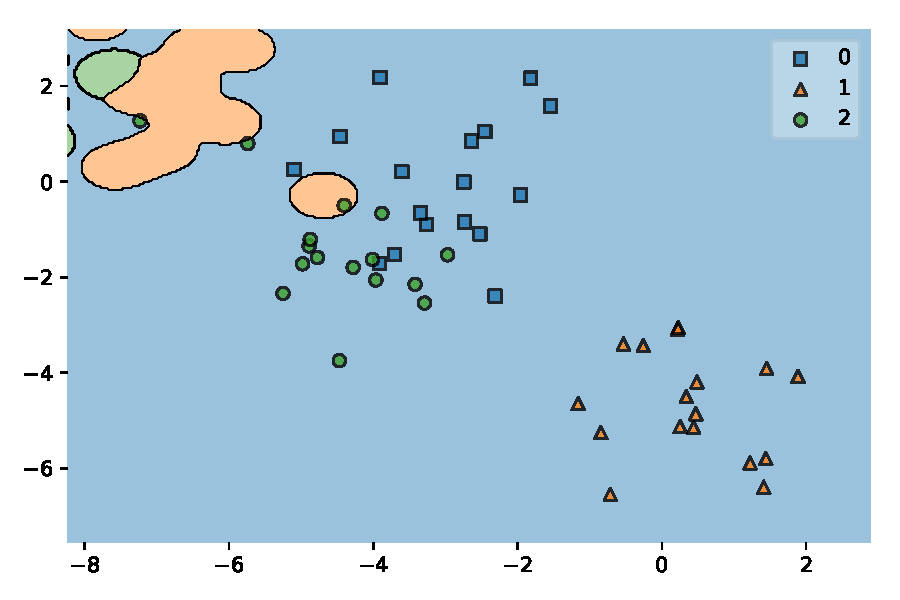
\includegraphics[width=1.0\textwidth]{imgs/underfit.pdf}
			\textbf{Underfit: } The model fails to recognise data pattern
		\column{0.33\textwidth}
			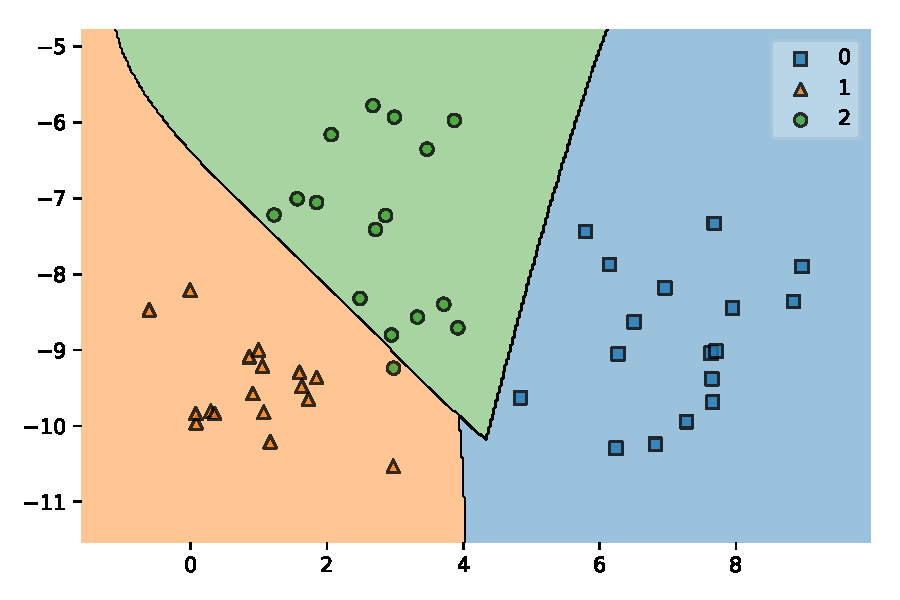
\includegraphics[width=1.0\textwidth]{imgs/good.pdf}
			\textbf{Good fit: } The model recognises data pattern \textbf{generally}
		\column{0.33\textwidth}
			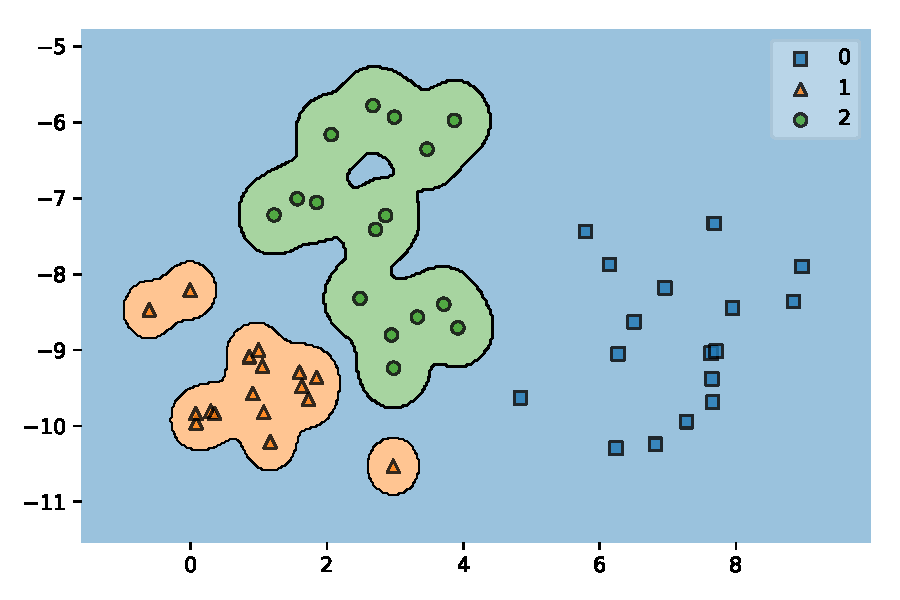
\includegraphics[width=1.0\textwidth]{imgs/overfit.pdf}
			\textbf{Overfit:} The model \textbf{remembers} data pattern instead of generalising.
	\end{columns}
\end{frame}

\begin{frame}
	\frametitle{Overfitting and underfitting}
	\begin{center}
		{\LARGE Good model must \textbf{generalise}}\\
	\end{center}
\end{frame}

\end{document}